\documentclass[a4paper,oneside,DIV=12,12pt,headings=normal]{scrartcl}

%%% Length calculations
\usepackage{calc}
%%%

%%% Support for color
\usepackage{xcolor}
\definecolor{lightblue}{HTML}{03A9F4}
\definecolor{red}{HTML}{F44336}
%%%

%%% Graphics inclusion
\usepackage{graphicx}
%%%

%%% Font selection
\usepackage{fontspec}

\setromanfont{STIX Two Text}[
	SmallCapsFeatures = {LetterSpace = 5},
]

\setsansfont{Source Sans Pro}[
]

\setmonofont{Source Code Pro}[
]
%%%

%%% Math settings
\usepackage{amsmath,unicode-math}
\setmathfont{STIX Two Math}

% \usepackage{IEEEtrantools}
\usepackage{mleftright}
%%%

%%% Font settings for different KOMA Script elements
\setkomafont{pagenumber}{\rmfamily}
\setkomafont{disposition}{\rmfamily\bfseries}
%%%

%%% Typographic enhancements
\usepackage{microtype}
%%%

%%% Language-specific settings
\usepackage{polyglossia}
\setmainlanguage{ukrainian}
%%%

%%% List settings
\usepackage{enumitem}
 \setlist[enumerate]{
	 noitemsep,
% 	leftmargin = *,
 }
%%%

%%% Captions
\usepackage{caption}
\usepackage{subcaption}

\DeclareCaptionLabelFormat{closing}{#2)}
\captionsetup[subtable]{labelformat = closing}
\captionsetup[subfigure]{labelformat = closing, position = auto}
%%%

%%% Tables
\usepackage{booktabs}
\usepackage{longtable}

\usepackage{multirow}

\usepackage{array}
\newcolumntype{v}[1]{>{\raggedright\arraybackslash\hspace{0pt}}p{#1}}
\newcolumntype{b}[1]{>{\centering\arraybackslash\hspace{0pt}}p{#1}}
\newcolumntype{n}[1]{>{\raggedleft\arraybackslash\hspace{0pt}}p{#1}}

\usepackage{kbordermatrix} % labeling array indices
%%%

%%% Floats on a single row
\usepackage{floatrow}
\newfloatcommand{capbtabbox}{table}[][\FBwidth]
%%%

%%% Physical units
\usepackage{siunitx}
%%%

%%% Set counters withing subsections
\usepackage{chngcntr}
\counterwithin{table}{subsection}
\counterwithin{figure}{subsection}
%%%

%%% Links and hyperreferences
\usepackage{hyperref}
\hypersetup{
	colorlinks      = false,
	linkbordercolor = red,
	urlbordercolor  = lightblue,
	pdfborderstyle  = {/S/U/W 1.5},
}
%%%

%%% All caps
\newcommand{\allcaps}[1]{{\addfontfeatures{LetterSpace = 3}#1}}
%%%

%%% Ceiling function typesetting
\newcommand{\ceil}[1]{\mleft\lceil#1\mright\rceil}
%%%

%%% Typesetting schematic elements
\newcommand{\schel}[1]{\textit{#1}}
%%%

%%% Shift operators
\DeclareMathOperator{\L1}{L1}
\DeclareMathOperator{\R1}{R1}
%%%

%%% Address intervals
\newcommand{\addrinterval}[2]{(#1{:}#2)}
%%%

\setlength{\emergencystretch}{1em}

\begin{document}
	\begin{titlepage}
	\centering
		Міністерство освіти і науки України\\
		Національний авіаційний університет\\
		Навчально-науковий інститут комп'ютерних інформаційних технологій\\
		Кафедра комп'ютеризованих систем управління

		\vspace*{\fill}

		Лабораторна робота №6\\
		з дисципліни «Архітектура комп'ютерів»\\
		на тему «Побудова блоку обробки даних»\\
		% Варіант №4

		\vspace*{\fill}
		
		\begin{flushright}
			Виконав:\\
			студент ННІКІТ СП-225\\
			Клокун В.\,Д.\\
			Перевірив:\\
			Зіньков Ю.\,Г.
		\end{flushright}

		Київ 2018
    \end{titlepage}

		\section{Мета роботи}
			Вивчення схемотехніки та системи мікрооперацій процесорного елементу~К1804ВС1, побудова блоку обробки даних на його основі та розробка мікропрограм обчислення функцій.

		\section{Завдання}
			При виконанні роботи ставляться такі завдання:
			\begin{enumerate}
				\item Розробити принципову схему блоку обробки даних на основі процесорного елементу~ВС1.
				\item Розробити алгоритми та мікропрограми обчислення функцій~(табл.~\ref{tab:task}), представити результати їх виконання: стани регістрів~\allcaps{RAM}, шини \allcaps{DO} та ін.
				\item Обчислити часові параметри мікрокоманд мікропрограми.
				\item Підготувати дані для прикладної програми «Емулятор~К1804ВС1».
			\end{enumerate}
			\begin{table}[!htbp]
				\centering
					\begin{tabular}{lrrrrrrrn{3em}n{3em}rrr}
						\toprule
							№ & Ф-ція & \multicolumn{3}{b{8em}}{Джерела операндів} & \multicolumn{3}{b{8em}}{Приймачі результату} & \multicolumn{2}{b{8em}}{Значення операндів} & \multicolumn{3}{c}{БОД} \\
							\cmidrule(lr){3-5} \cmidrule(lr){6-8} \cmidrule(lr){9-10} \cmidrule(lr){11-13}
								&         & \schel{RAM[i]} & \schel{D1} & \schel{Q} & \schel{RAM(i)} & \schel{Q} & \schel{DO} & $x_2$ & $x_1$ & $n$ & \schel{BP1} & \schel{RGC} \\
						\midrule
							4 &  3 & $6(X_2)$ & $x_1$ &       & 7  & & + & $4$ &  $3$ & 16 & + & + \\
							4 & 13 & $5(X_2)$ &       & $x_1$ & 10 & & + & $3$ & $-2$ & 16 & + & + \\
						\bottomrule
					\end{tabular}
				\caption{Завдання}
				\label{tab:task}
			\end{table}

		\section{Хід роботи}
			\subsection{Процесорний елемент~К1804ВС1}
				Процесорний елемент~ВС1~(структурна схема на рис.~\ref{fig:vs1-struct-schematic}) має 4-розрядну організацію. Його використовують для побудови операційних блоків процесорів з довільною розрядністю. Блок внутрішньої пам'яті містить в собі 2-портовий регістровий запам'ятовуючий пристрій з організацією~\allcaps{RAM} ємністю 16~4-розрядних слів та зміщувач даних \schel{SHL1}.
				\begin{figure}[!htbp]
					\centering
					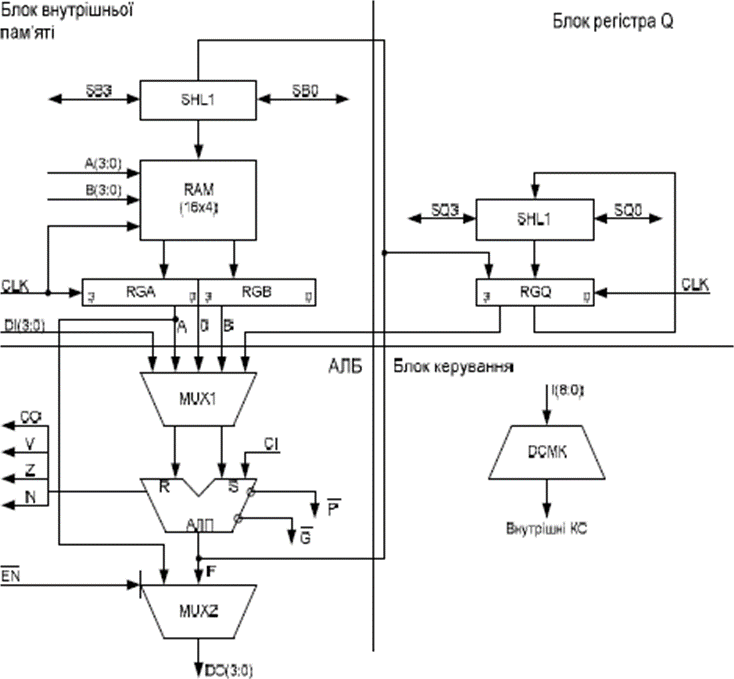
\includegraphics[height = 14\baselineskip]{./assets/01-vs1-structure.png}
					\caption{Структура процесорного елемента~К1804ВС1}
					\label{fig:vs1-struct-schematic}
				\end{figure}
				
				Вибір довільного регістра в якості джерела інформації виконують шляхом задання його адреси на входах~$A~\addrinterval{3}{0}$~(порт~\schel{A}) або~$B~\addrinterval{3}{0}$~(порт~\schel{B}). Є можливість одночасного зчитування двох слів із~\allcaps{RAM}. Зчитані дані заносять в регістри~\schel{RGA} та~\schel{RGB}. Запис даних в~\allcaps{RAM} можливий тільки за адресою~$\schel{B}~\addrinterval{3}{0}$ під час переходу тактового сигналу~\schel{CLK} зі стану «1» в стан «0». Можна записувати інформацію в~\allcaps{RAM} як без зсуву, так і зі зсувом вправо або вліво на 1~розряд. Сигнали~\schel{SB3}, \schel{SB0} виникають на однойменних двонаправлених виводах процесорного елемента при виконанні операції зсуву даних перед їх записом в~\allcaps{RAM}. Якщо зсуви на зміщувачі~\schel{SHL1} не виконуються, то вказані виводи перебувають у третьому стані.

				Арифметично-логічний блок складається з мультиплексора вибору даних~\schel{MUX1}, арифметично-логічного пристрою та мультиплексора вихідних даних~\schel{MUX2}. Функції, які реалізує арифметично-логічний пристрій, визначаються мікрокодом~$I~\addrinterval{8}{0}$, який дешифрується в блоці керування. При цьому формуються внутрішні керуючі сигнали. Мультиплексор~\schel{MUX1} забезпечує вибір пар операндів на входах ариф\-ме\-тич\-но-ло\-гіч\-но\-го пристрою~\schel{R} та~\schel{S}. Джерелами операндів арифметично-логічного пристрою є:
				\begin{enumerate}
					\item Зовнішня шина даних~$\schel{DI}~\addrinterval{3}{0}$.
					\item Константа «0».
					\item Регістр~\schel{RGQ}.
					\item Регістри \allcaps{RAM}, зчитані з каналів~\schel{A} та~\schel{B}.
				\end{enumerate}
				Керування вибором пар операндів забезпечується полем~$\schel{I}~\addrinterval{2}{0}$~(табл.~\ref{tab:operand-sources}).
				\begin{table}[!htbp]
					\centering
					\begin{tabular}{*{6}{c}}
						\toprule
							\multicolumn{4}{c}{$\schel{I}~\addrinterval{2}{0}$} & \multicolumn{2}{c}{Виходи АЛП}\\
							\cmidrule(lr){1-4} \cmidrule(lr){5-6}
							12 & 11 & 10 & 8-а с.о. & $R$ & $S$ \\
						\midrule
							0  & 0  & 0  & C        & $A$ & $Q$ \\
							0  & 0  & 1  & 1        & $A$ & $Q$ \\
							0  & 1  & 0  & 2        & $0$ & $Q$ \\
							0  & 1  & 1  & 3        & $0$ & $Q$ \\
							1  & 0  & 0  & 4        & $0$ & $Q$ \\
							1  & 0  & 1  & 5        & $D$ & $Q$ \\
							1  & 1  & 0  & 6        & $D$ & $Q$ \\
							1  & 1  & 1  & 7        & $D$ & $Q$ \\
						\bottomrule
					\end{tabular}
					\caption{Джерела операндів}
					\label{tab:operand-sources}
				\end{table}

				Арифметично-логічний пристрій виконує вісім арифметичних та логічних операцій. Тип операцій в арифметично-логічному пристрої задається полем мікрокоманди~$\schel{I}~\addrinterval{5}{3}$, а їх список визначається за визначеними правилами~(табл.~\ref{tab:alu-operations}). Арифметичні операції виконують з урахуванням значення вхідного переносу~\schel{CI} за правилами доповнювального коду. При цьому формуються 4~ознаки результату:
				\begin{enumerate}
					\item \schel{CO} — перенесення зі старшого розряду.
					\item \schel{V} — переповнення.
					\item \schel{N} — знак або вміст старшого розряду на виході арифметично-логічного пристрою.
					\item \schel{Z} — ознака нульового значення~\schel{F} на виході арифметично-логічного пристрою.
				\end{enumerate}
				Крім того формуються сигнали генерації~\schel{G} та розповсюдження (поширення) переносу~\schel{P} в арифметико-логічному пристрої, які потрібні для організації прискореного переносу в багаторозрядній схемі, яка побудована із кількох процесорних елементів.
				\begin{table}[!htbp]
					\centering
					\begin{tabular}{*{5}{l}}
						\toprule
							\multicolumn{4}{c}{$\schel{I}~\addrinterval{5}{3}$} & Операція\\
							\cmidrule(lr){1-4}
							15 & 14 & 13 & 8-а о.о. &  \\
						\midrule
							0  & 0  & 0  & 0        & $R + S + CI$ \\
							0  & 0  & 1  & 1        & $S - R - 1 + CI$ \\
							0  & 1  & 0  & 2        & $R - S - 1 + CI$ \\
							0  & 1  & 1  & 3        & $R \lor S$ \\
							1  & 0  & 0  & 4        & $R \land S$ \\
							1  & 0  & 1  & 5        & $\neg R \land S$ \\
							1  & 1  & 0  & 6        & $R \oplus S$ \\
							1  & 1  & 1  & 7        & $\neg ( R \oplus S)$\\
						\bottomrule
					\end{tabular}
					\caption{Операції в арифметично-логічному пристрої}
					\label{tab:alu-operations}
				\end{table}


				Результат операції на виході арифметично-логічного пристрою задається словом~$F$ та видається в шину~\schel{DO}, в~\allcaps{RAM} або регістр~\schel{RGQ} відповідно до розрядів мікрокоду~$\schel{I}~\addrinterval{8}{6}$~(табл.~\ref{tab:result-destinations}). Запис слова~$F$ в~\allcaps{RAM} здійснюється через канал~\schel{B} прямо~($\schel{RAM}[B] = F$), зсувом вправо~($\schel{RAM}[B] = \R1 (F)$) або зсувом вліво~($\schel{RAM}[B] = \L1 (F)$). В двох останніх випадках одночасно може зсуватись і вміст регістра~\schel{RGQ}: ($\schel{RGQ} = \R1(\schel{RGQ})$ або~$\schel{RGQ} = \L1(\schel{RGQ})$).
				\begin{table}[!htbp]
					\centering
					\begin{tabular}{*{7}{r}}
						\toprule
							\multicolumn{4}{c}{$\schel{I}~\addrinterval{8}{6}$} & \\
							\cmidrule(lr){1-4}
							8 & 7 & 6 & 8-а о.о. & $RAM[B]$ & \schel{RGQ} & \schel{DO} \\
						\midrule
							0 & 0 & 0 & 0        &          & $F$        & $F$ \\ 
							0 & 0 & 1 & 1        &          &            & $F$ \\ 
							0 & 1 & 0 & 2        & $F$      &            & $A$ \\ 
							0 & 1 & 1 & 3        & $F$      &            & $F$ \\ 
							1 & 0 & 0 & 4        & $\R1(F)$ & $\R1(RGQ)$ & $F$ \\ 
							1 & 0 & 1 & 5        & $\R1(F)$ &            & $F$ \\ 
							1 & 1 & 0 & 6        & $\R1(F)$ & $\R1(RGQ)$ & $F$ \\ 
							1 & 1 & 1 & 7        & $\R1(F)$ &            & $F$ \\ 
						\bottomrule
					\end{tabular}
					\caption{Приймачі результату}
					\label{tab:result-destinations}
				\end{table}

				Мультиплексор~\schel{MUX2} забезпечує передачу слова~$F$ з виходу ариф\-ме\-тич\-но-логіч\-но\-го пристрою або виходу~$A$ на вихідну шину~$\schel{DO}~\addrinterval{3}{0}$. Блок регістра~$Q$ складається з регістра~\schel{RGQ} та зміщувача~\schel{SHL2}. Регістр~\schel{RGQ} забезпечує прийом слова~$F$~($\schel{RGQ} = F$) та зсув свого вмісту на один розряд вліво~($\schel{RGQ} = \L1(\schel{RGQ})$) або вправо~($\schel{RGQ} = \L1(\schel{RGQ})$) за допомогою зміщувача~\schel{SHL2}. Сигнали~\schel{SQ3}, \schel{SQ0} виникають на однойменних двонапрямлених виводах процесорного елемента при зсуві інформації в регістрі~\schel{RGQ}. Якщо зсув не виконується, то вказані виводи знаходяться в третьому стані. Запис інформації в регістр~\schel{RGQ} виконується при переході тактового сигналу~\schel{SCL} зі стану «0» в «1».

				Блок керування формує внутрішні керуючі сигнали шляхом декодування відповідних полів мікрокода:
				\begin{equation*}
					I(8{:}0) = I(8{:}6).I(5{:}3).I(2{:}0),
				\end{equation*}
				де $I(8{:}0)$~— поле вибору пари джерел операндів, $I(8{:}0)$~— поле операції в ариф\-ме\-тич\-но-логіч\-но\-му пристрої, $I(8{:}0)$~— поле вибору приймача результату.

				Процесорний елемент ВС1~(умовно-графічне позначення на рис.~\ref{fig:vs1-mark}, призначення виводів у табл.~\ref{tab:vs1-out-description}) виконаний у пластмасовому корпусі типу~2123.40-17.
				\begin{figure}[!htbp]
					\centering
					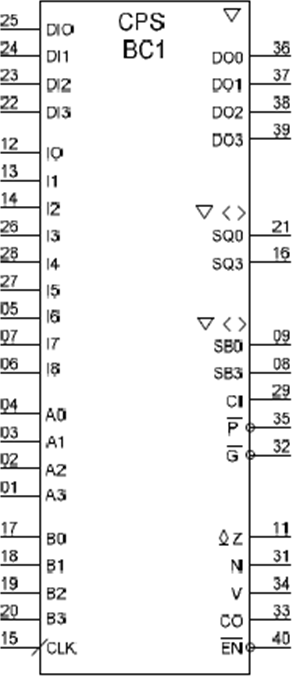
\includegraphics[height = 13\baselineskip]{./assets/02-vs1-mark.png}
					\caption{Умовно-графічне позначення процесорного елемента К1804ВС1}
					\label{fig:vs1-mark}
				\end{figure}

				\begin{table}[!htbp]
					\centering
					\begin{tabular}{v{6em}ll}
						\toprule
							Виводи & Позначення & Призначення \\
						\midrule
							1–4   & \schel{A3}—\schel{A0} & Входи адреси~\allcaps{RAM} по каналу~$A$ \\
							20–17 & \schel{B3}—\schel{B0} & Входи адреси~\allcaps{RAM} по каналу~$B$ \\
							6, 7, 5, 27, 28, 25, 14, 13, 12 & \schel{A4}—\schel{A0} & Входи мікрокоду~$I~\addrinterval{8}{0}$ \\
							22–26 & \schel{DI3}—\schel{DI0} & Входи даних \\
							30–36 & \schel{DO3}—\schel{DO0} & Виходи даних\\
							15    & \schel{CLK}             & Тактові сигнали \\
							21    & \schel{SQ0}             & Вхід/вихід молодшого розряду зміщувача~\schel{SHL2} \\
							16    & \schel{SQ3}             & Вхід/вихід старшого розряду зміщувача~\schel{SHL2} \\
							9     & \schel{SB0}             & Вхід/вихід молодшого розряду зміщувача~\schel{SHL1} \\
							8     & \schel{SB3}             & Вхід/вихід старшого розряду зміщувача~\schel{SHL1} \\
							29    & \schel{CI}              & Вхід переносу в~АЛП \\
							32, 35 & $\overline{P}$, $\overline{G}$ & Виходи прискореного переносу \\
							11    & \schel{Z}               & Вихід ознаки нульового результату в~АЛП \\
							31    & \schel{N}               & Вихід старшого розряду~АЛП \\
							34    & \schel{V}               & Вихід ознаки переповнення результату \\
							33    & \schel{CO}              & Вихід переносу з~АЛП \\
							40    & $\overline{EN}$         & Вхід дозволу видачі даних~\schel{DO} \\
							10    & $U_{\mathrm{cc}}$                & \SI{5}{\volt} \\
							1–4   & \schel{GND}             & Загальний \\
						\bottomrule
					\end{tabular}
					\caption{Виводи процесорного елемента К1804ВС1}
					\label{tab:vs1-out-description}
				\end{table}

			\subsection{Побудова блоку обробки даних}
				Необхідна довжина розрядної сітки процесора забезпечується шляхом з'єднання кількох процесорних елементів~ВС1~(рис.~\ref{fig:vs1-cascade}) за умови, що $n = 16$. Шини~\schel{A}, \schel{B} та~\schel{I} підключаються паралельно при кожному процесорному елементі~ВС1 аналогічно лініями~\schel{EN} та~\schel{CLK}. Вихід переносу~\schel{CO} молодшого процесорного елемента~\schel{DD1} підключається до входу переносу~\schel{CI} процесорного елемента~\schel{DD2} і так далі. Послідовна передача переносу між процесорними елементами~ВС1 знижує швидкодію процесора. Для прискорення поширення переносу використовуються інтегральна мікросхема К1804ВР1. Виходи ознак~\schel{CO}, \schel{F15}, \schel{V}, \schel{Z}~(процесорний елемент~\schel{DD4}) підключаються до регістра стану~\schel{RGC}.
				\begin{figure}[!htbp]
					\centering
					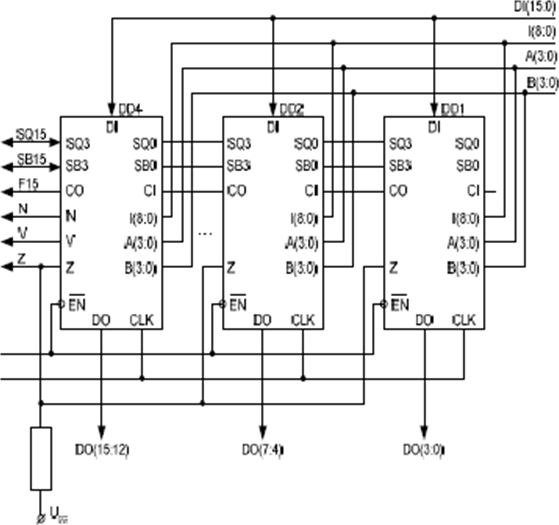
\includegraphics[height = 15\baselineskip]{./assets/03-vs1-cascade.png}
					\caption{Об'єднання процесорних елементів ВС1 при послідовному поширенні переносу}
					\label{fig:vs1-cascade}
				\end{figure}

				В блок дані поступають із шини~$\schel{DI}~\addrinterval{15}{0}$. Результат перетворення видається на шину даних~$\schel{DO}~\addrinterval{15}{0}$. Керування 16-розрядним операційним блоком процесора відбувається за допомогою макрокоманди:
				\begin{equation*}
					I~\addrinterval{8}{0}.B~\addrinterval{3}{0}.A~\addrinterval{3}{0}.\overline{EN}.\schel{SQ15}.\schel{SQ0}.\schel{SB15}.\schel{SB0}.\schel{CI},
				\end{equation*}
				де $I~\addrinterval{8}{0}$~— мікрокод, який керує роботою процесорного елемента, $B~\addrinterval{3}{0}$, $A~\addrinterval{3}{0}$~— адреси регістрів~\allcaps{RAM} на входах портів~$B$ та~$A$, \schel{CI}~— однобітне поле, яке визначає значення сигналу на одноіменному вході процесорного елемента.

			\subsection{Схема прискореного переносу К1804ВР1}
				Схема прискореного переносу ВР1~(умовно-графічне позначення на~рис.~\ref{fig:vs1-fast-shift}, виводи у табл.~\ref{tab:vs1-fast-shift-outs}) служить для організації ланцюга паралельного переносу в 16-розрядних процесорах, побудованих на базі 4~процесорних елементів ВС1. Були розроблені схеми з'єднання процесорних елементів~ВС1 при використанні схем прискореного переносу~ВР1 для~$n = 16$~(рис.~\ref{fig:vs1-data-processing-block-fast-shift}) та~$n = 32$~(рис.~\ref{fig:vs1-data-processing-block-fast-shift-cascade}).
				\begin{figure}[!htbp]
					\centering
					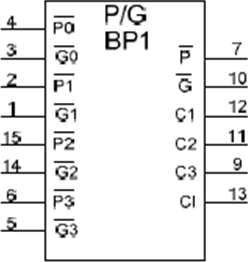
\includegraphics[height = 7\baselineskip]{./assets/04-vs1-fast-shift.png}
					\caption{Умовно-графічне позначення схеми прискореного переносу ВР1}
					\label{fig:vs1-fast-shift}
				\end{figure}

				\begin{table}[!htbp]
					\centering
					\begin{tabular}{lll}
						\toprule
							Виводи & Позначення & Призначення \\
						\midrule
							4, 2, 15, 6 & $\overline{P0}$, $\overline{P3}$ & Входи розповсюдження переносу \\
							3, 1, 14, 5 & $\overline{G0}$, $\overline{G3}$ & Входи генерації переносу \\
							7, 10       & $\overline{P}$, $\overline{G}$   & Входи розповсюдження і генерації переносу \\
							12, 11, 9   & $C1$, $C2$, $C3$                 & Входи переносу молодшої, середньої та старшої груп\\
							18          & \schel{CI}                       & Вхідний переніс \\
							16          & $U_{\mathrm{cc}}$                & \SI{5}{\volt} \\
							8           & \schel{GND}                      & \\
						\bottomrule
					\end{tabular}
					\caption{Виводи схеми прискореного переносу В1804ВР1}
					\label{tab:vs1-fast-shift-outs}
				\end{table}

				\begin{figure}[!htbp]
					\centering
					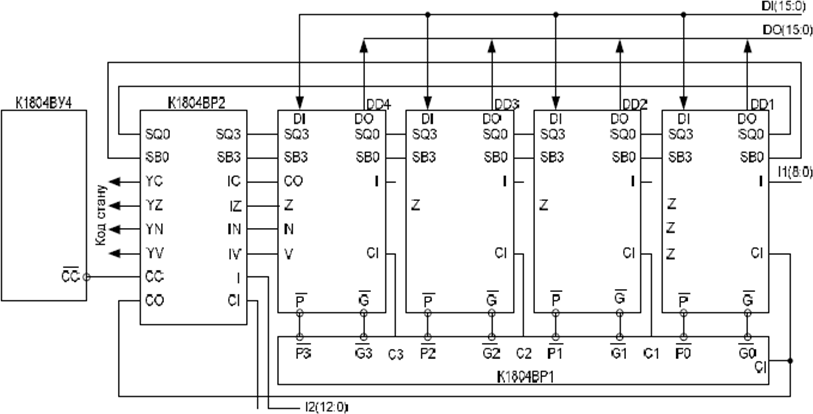
\includegraphics[height = 12\baselineskip]{./assets/05-vs1-data-processing-block-fast-shift.png}
					\caption{Блок обробки даних з використанням схеми прискореного переносу ВР1 для~$n = 16$}
					\label{fig:vs1-data-processing-block-fast-shift}
				\end{figure}

				\begin{figure}[!htbp]
					\centering
					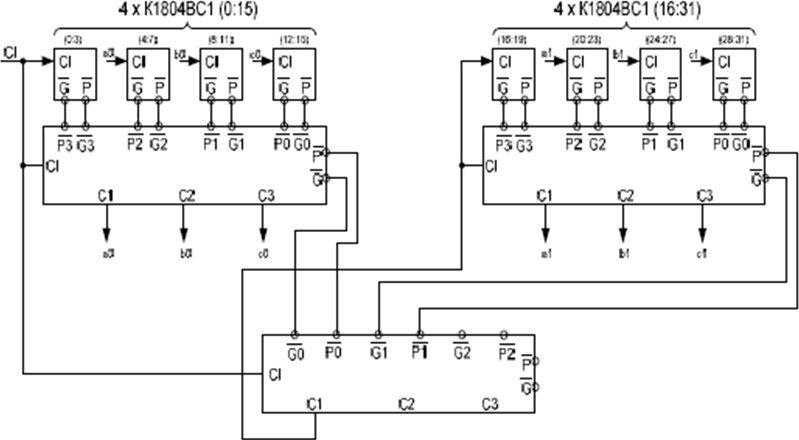
\includegraphics[height = 12\baselineskip]{./assets/06-vs1-data-processing-block-fast-shift-cascade.png}
					\caption{Каскадне з'єднання схем прискореного переносу ВР1}
					\label{fig:vs1-data-processing-block-fast-shift-cascade}
				\end{figure}

				Для обчислення швидкодії блоку обробки даних наведемо часові характеристики мікросхем~К1804ВС1 та~К1804ВР1~(табл.~\ref{tab:vs1-time-params}).
				\begin{table}[!htbp]
					\centering
					\begin{tabular}{llr}
						\toprule
							Звідки & Куди & Значення, нс \\
						\midrule
							% \multicolumn{3}{c}{\emph{Затримки сигналів}} \\
							$A(B)$ & $DO, N$                      & 85 \\
							$A(B)$ & $CO$                         & 80 \\
							$A(B)$ & $V$                          & 90 \\
							$A(B)$ & $\overline{P}, \overline{G}$ & 70 \\
							$A(B)$ & \schel{SB3}, \schel{SB0}     & 100 \\
							$I$    & $DO, CO, N$                  & 80 \\
							$I$    & $V, Z$                       & 70 \\
							$I$    & \schel{SB3, SB0, SQ3, SQ0}   & 35 \\
							$DI$   & $DO, N, CO$                  & 50 \\
							$DI$   & \schel{SB3, SB0}             & 70 \\
							$DI$   & $\overline{P}, \overline{G}$ & 40 \\
							$CI$   & $DO, N$                      & 35 \\
							$CI$   & $CO$                         & 25 \\
							$CI$   & $Z, \schel{SB3, SB0}$        & 55 \\
							\multicolumn{2}{l}{Тривалість сигналу~\schel{CLK}} & 30 \\
						\bottomrule
					\end{tabular}
					\caption{Часові параметри мікросхеми К1804ВС1}
					\label{tab:vs1-time-params}
				\end{table}

			\subsection{Стани регістрів}
				Після виконання роботи та виконання необхідних операцій перевіряємо значення регістрів~(табл.~\ref{tab:registers-state}).
				\begin{table}[!htbp]
					\centering
						\begin{tabular}{lr}
							\toprule
								Регістр & Стан \\
							\midrule
								\schel{R0}   & 000008 \\
								\schel{R1}   & 000004 \\
								\schel{R2}   & 000000 \\
								\schel{R3}   & 000000 \\
								\schel{R4}   & 000000 \\
								\schel{R5}   & 000000 \\
								\schel{R6}   & 000000 \\
								\schel{R7}   & 000000 \\
								\schel{R8}   & 000000 \\
								\schel{R9}   & 000000 \\
								\schel{R10}  & 000000 \\
								\schel{R11}  & 000000 \\
								\schel{R12}  & 000000 \\
								\schel{R13}  & 000000 \\
								\schel{R14}  & 000000 \\
								\schel{R15}  & 000000 \\
								\schel{DO}   & 000004 \\
								\schel{RO}   & 000004 \\
								\schel{CO}   & 0 \\
								\schel{F15}  & 0 \\
								\schel{SQ15} & 0 \\
								\schel{SB15} & 0 \\
								\schel{SQO}  & 0 \\
								\schel{SBO}  & 0 \\
								\schel{DO}   & 0 \\
							\bottomrule
						\end{tabular}
					\caption{Стан регістрів}
					\label{tab:registers-state}
				\end{table}

		\section{Висновок}
			Під час виконання даної лабораторної роботи ми вивчили схемотехніку та систему мікрооперацій процесорного елементу~К1804ВС1, побудували блок обробки даних на його основі та розробили мікропрограми обчислення функцій.


\end{document}

